\documentclass[a4paper]{article}
\usepackage{geometry}
\usepackage{graphicx}
\usepackage{natbib}
\usepackage{amsmath}
\usepackage{amssymb}
\usepackage{amsthm}
\usepackage{paralist}
\usepackage{epstopdf}
\usepackage{tabularx}
\usepackage{longtable}
\usepackage{multirow}
\usepackage{multicol}
\usepackage[hidelinks]{hyperref}
\usepackage{fancyvrb}
\usepackage{algorithm}
\usepackage{algorithmic}
\usepackage{float}
\usepackage{paralist}
\usepackage[svgname]{xcolor}
\usepackage{enumerate}
\usepackage{array}
\usepackage{times}
\usepackage{url}
\usepackage{fancyhdr}
\usepackage{comment}
\usepackage{environ}
\usepackage{times}
\usepackage{textcomp}
\usepackage{caption}
\usepackage{tikz}
\usetikzlibrary{patterns}
\usetikzlibrary{shapes,backgrounds}



\urlstyle{rm}

\setlength\parindent{0pt} % Removes all indentation from paragraphs
\theoremstyle{definition}
\newtheorem{definition}{Definition}[]
\newtheorem{conjecture}{Conjecture}[]
\newtheorem{example}{Example}[]
\newtheorem{theorem}{Theorem}[]
\newtheorem{lemma}{Lemma}
\newtheorem{proposition}{Proposition}
\newtheorem{corollary}{Corollary}

\floatname{algorithm}{Procedure}
\renewcommand{\algorithmicrequire}{\textbf{Input:}}
\renewcommand{\algorithmicensure}{\textbf{Output:}}
\newcommand{\abs}[1]{\lvert#1\rvert}
\newcommand{\norm}[1]{\lVert#1\rVert}
\newcommand{\RR}{\mathbb{R}}
\newcommand{\CC}{\mathbb{C}}
\newcommand{\Nat}{\mathbb{N}}
\newcommand{\br}[1]{\{#1\}}
\DeclareMathOperator*{\argmin}{arg\,min}
\DeclareMathOperator*{\argmax}{arg\,max}
\renewcommand{\qedsymbol}{$\blacksquare$}

\definecolor{dkgreen}{rgb}{0,0.6,0}
\definecolor{gray}{rgb}{0.5,0.5,0.5}
\definecolor{mauve}{rgb}{0.58,0,0.82}
% Define a macro for partial derivative
\newcommand{\pd}[2]{\frac{\partial #1}{\partial #2}}
\newcommand{\Var}{\mathrm{Var}}
\newcommand{\Cov}{\mathrm{Cov}}

\newcommand{\vc}[1]{\boldsymbol{#1}}
\newcommand{\xv}{\vc{x}}
\newcommand{\Sigmav}{\vc{\Sigma}}
\newcommand{\alphav}{\vc{\alpha}}
\newcommand{\muv}{\vc{\mu}}

\newcommand{\red}[1]{\textcolor{red}{#1}}

\def\x{\mathbf x}
\def\y{\mathbf y}
\def\w{\mathbf w}
\def\v{\mathbf v}
\def\E{\mathbb E}
\def\V{\mathbb V}

% TO SHOW SOLUTIONS, include following (else comment out):
\newenvironment{soln}{
	\leavevmode\color{blue}\ignorespaces
}{}


\hypersetup{
	%    colorlinks,
	linkcolor={red!50!black},
	citecolor={blue!50!black},
	urlcolor={blue!80!black}
}

\geometry{
	top=1in,            % <-- you want to adjust this
	inner=1in,
	outer=1in,
	bottom=1in,
	headheight=3em,       % <-- and this
	headsep=2em,          % <-- and this
	footskip=3em,
}


\pagestyle{fancyplain}
\lhead{\fancyplain{}{Homework 1}}
\rhead{\fancyplain{}{CS 760 Machine Learning}}
\cfoot{\thepage}

\title{\textsc{Homework 1}} % Title

%%% NOTE:  Replace 'NAME HERE' etc., and delete any "\red{}" wrappers (so it won't show up as red)

\author{
	\red{Huzaifa Mustafa Unjhawala} \\
	\red{9081963267}\\
} 

\date{}

\begin{document}
	
	\maketitle 
	
	
	\section{Vectors and Matrices [6 pts]}
	Consider the matrix $X$ and the vectors $\mathbf{y}$ and $\textbf{z}$ below:
	$$
	X = \begin{pmatrix}
		3 & 2 \\ -7 & -5 \\
	\end{pmatrix}
	\qquad \mathbf{y} = \begin{pmatrix}
		2 \\ 1
	\end{pmatrix} \qquad \mathbf{z} = \begin{pmatrix}
		1 \\ -1
	\end{pmatrix}
	$$
	\begin{enumerate}
		\item 	Compute $\mathbf{y}^{T} X \mathbf{z}$\\
			    \begin{soln} [0] \end{soln}
		\item 	Is $X$ invertible? If so, give the inverse, and if no, explain why not.\\
		        \begin{soln}  
					$|X| = -0.99 \neq 0$ therefore it is invertible. Its inverse is \\
					\[
						\begin{pmatrix}
							-5 & 2 \\ -7 & -3 \\
						\end{pmatrix}
					\]
				\end{soln}
	\end{enumerate}
	
	
	\section{Calculus [3 pts]}
	\begin{enumerate}
		\item If $y = e^{-x} + \arctan(z)x^{6/z} - \ln\cfrac{x}{x+1}$, what is the partial derivative of $y$ with respect to $x$?\\
		\begin{soln}
			\begin{align*}
				\pd{y}{x} &= -e^{-x} + \arctan(z) \frac{6}{z} x^{\frac{6}{z} - 1} - \frac{(x+1)}{x}\frac{(x+1-x)}{(x+1)^2} \\
						 &= -e^{-x} + \arctan(z) \frac{6}{z} x^{\frac{6}{z} - 1} - \frac{1}{x(x+1)}
			\end{align*}
		\end{soln}
	\end{enumerate}
	
	
	
	
	\section{Probability and Statistics [10 pts]}
	Consider a sequence of data $S = (1, 1, 1, 0, 1)$ created by flipping a coin $x$ five times, where 0 denotes that the coin turned up heads and 1 denotes that it turned up tails.
	\begin{enumerate}
		\item 	(2.5 pts) What is the probability of observing this data, assuming it was generated by flipping a biased coin with $p(x=1) = 0.6$?
		
		\begin{soln}  
			Assuming i.i.d,
			\begin{align*}
				P(S) &= P(x_1 = 1) \times P(x_2 = 1) \times P(x_3 = 1) \times P(x_4 = 0) \times P(x_5 = 1) \\
					 &= 0.6 \times 0.6 \times 0.6 \times 0.4 \times 0.6 \\
					 &= 0.05184
			\end{align*}
		\end{soln}
		
		\item 	(2.5 pts) Note that the probability of this data sample could be greater if the value of $p(x = 1)$ was not $0.6$, but instead some other value. What is the value that maximizes the probability of $S$? Please justify your answer.\\
		\begin{soln}
			Let $p$ be the probability of getting a head. Thus the probability of getting a tail is $1-p$. Then, 
			\begin{align*}
				P(S) &= P(x_1 = 1) \times P(x_2 = 1) \times P(x_3 = 1) \times P(x_4 = 0) \times P(x_5 = 1) \\
					 &= p^4(1-p)
			\end{align*}
			Taking the first derivative and equating to 0,
			\begin{align*}
				\pd{P(s)}{p} &= 4p^3(1-p) - p^4 \\
							&= p^3(4-5p) \\
			\end{align*}
			Equating this to 0, we get $p = 0$ or $p = \frac{4}{5}$. Since $p = 0$ is not possible, the value that maximizes the probability of $S$ is $p = \frac{4}{5}$.

		\end{soln}
		
		\item 	(5 pts) Consider the following joint probability table where both $A$ and $B$ are binary random variables: 
		\begin{table}[htb]
			\centering
			\begin{tabular}{ccc}\hline
				A & B & $P(A, B)$  \\\hline
				0 & 0 & 0.3 \\
				0 & 1 & 0.1 \\
				1 & 0 & 0.1 \\
				1 & 1 & 0.5 \\\hline
			\end{tabular}
		\end{table}
		\begin{enumerate}
			\item 	What is $P(A = 0 | B = 1)$?\\
			 \begin{soln}
				\begin{align*}
					P(A,B) &= P(B)P(A|B)\\
					\implies P(A|B) &= \frac{P(A,B)}{P(B)} \\
									&= \frac{P(A=0,B=1)}{P(B=1)} \\
									&= \frac{0.1}{P(A=0,B=1) + P(A=1,B=1)} \\
								 	&= \frac{0.1}{0.1 + 0.5} \\
								 	&= \frac{1}{6}
				\end{align*}
			 \end{soln}
			 
			\item 	What is $P(A = 1 \vee B = 1 )$?\\
			\begin{soln}
				\begin{align*}
					P(A=1 \vee B=1) &= P(A=1) + P(B=1) - P(A=1,B=1) \\
									&= P(A=1,B=0) + P(A=1,B=1) + P(A=0,B=1) + P(A=1,B=1) - 0.5 \\
									&= 0.1 + 0.5 + 0.1 + 0.5 - 0.5 \\
									&= 0.7
				\end{align*}
			
			\end{soln}
		\end{enumerate}
	\end{enumerate}
	
	
	\section{Big-O Notation [6 pts]}
	For each pair $(f, g)$ of functions below, list which of the following
	are true: $f(n) = O(g(n))$, $g(n) = O(f(n))$, both, or
	neither. Briefly justify your answers.
	\begin{enumerate}
		\item 	$f(n) = \ln(n)$, $g(n) = \log_{2}(n)$.\\
		\begin{soln}
			$log_{2}(n) = \frac{ln(n)}{ln(2)}$ \\
			Therefore $f(n) = O(g(n))$ as $ln(2)$ is a constant \\
			Similarly, $ln(n) = \frac{log_2(n)}{log_2(e)}$, thus, $g(n) = O(f(n))$.
		\end{soln}
		
		\item 	$f(n) =  \log_{2}\log_{2}(n)$, $g(n) = \log_{2}(n)$.\\
		
		\begin{soln}  
			$f(n) = log_2(g(n))$, thus $f(n) \ne O(g(n))$ and vice versa.\\	
		\end{soln}
		
		\item 	$f(n) = n!$, $g(n) = 2^n$.\\
		\begin{soln}
		$f(n) \ne O(g(n))$ and vice versa as $n!$ grows faster than $2^n$. This is intuitve as $n!$ is n factors multiplied together while $2^n$ is just $n$ factors of 2 multiplied together. Thus asymptotically, $2^n$ is bigger\\
		\end{soln}
	\end{enumerate}
	
	
	
	
	
	\section{Probability and Random Variables }
	\subsection{Probability [12.5 pts]}
	State true or false. Here $\Omega$ denotes the sample space and $A^c$ denotes the complement of the event $A$.
	\begin{enumerate}
		\item For any $A, B \subseteq \Omega$, $P(A|B)P(A) = P(B|A)P(B)$.\\
		\begin{soln}
			False. 
			\begin{align*}
				&P(B|A) = P(A,B)/P(A) \\
				\implies &P(B|A)P(A) = P(A,B) \\
			\end{align*}
			Similarly,
			\begin{align*}
				P(A|B)P(B) &= P(A,B) \\
			\end{align*}
			Thus, $P(A|B)P(A) \ne P(B|A)P(B)$
		
		\end{soln}
		
		\item For any $A, B \subseteq \Omega$, $P(A \cup B) = P(A) + P(B) - P(B \cap A)$.\\         
		\begin{soln}  
			True. Can  be shown with a venn diagram. Its a law of probability.
		\end{soln}
		
		\item For any $A, B, C \subseteq \Omega$ such that $P(B \cup C) > 0$,
		$\frac{P(A \cup B \cup C)}{P(B \cup C)} \geq P(A | B \cup C) P(B)$.\\ 
		\begin{soln}
			True. Through Bayes, 
			\begin{align}
				P(A|B \cup C) &= \frac{P(A,B \cup C)}{P(B \cup C)} \\
				&= \frac{P(A,B) + P(A,C) - P(A,B,C)}{P(B \cup C)} \\
				P(A|B \cup C) P(B)&= \frac{P(A,B)P(B) + P(A,C)P(B) - P(A,B,C)P(B)}{P(B \cup C)}
			\end{align}
			Now, we need to show $P(A \cup B \cup C) \ge P(A,B)P(B) + P(A,C)P(B) - P(A,B,C)P(B)$. See venn diagram below, \\
			\begin{tikzpicture}
				% Define the circles
				\node[draw, circle, minimum size=4cm] (A) at (0,0) {A};
				\node[draw, circle, minimum size=4cm] (B) at (3,0) {B};
				\node[draw, circle, minimum size=4cm] (C) at (1.5,-2.5) {C};
			  
				% Label the circles
				\node[above] at (A.north) {A};
				\node[above] at (B.north) {B};
				\node[below] at (C.south) {C};	
			\end{tikzpicture}

			The red and green shaded regions represent $P(A,B) + P(B,C)$ and $P(A,B,C)$ respectively. Thus the numerator of the RHS on Eq.3 is just the red region without the intersection $P(A,B,C)$. This is much lesser than $P(A \cup B \cup C)$. Since $P(B) \le 1$, $P(A \cup B \cup C) \ge P(A,B)P(B) + P(A,C)P(B) - P(A,B,C)P(B)$.
		\end{soln}
		
		\item For any $A, B\subseteq\Omega$ such that $P(B) > 0, P(A^c) > 0$,
		$P(B|A^C) + P(B|A) = 1$.\\ 
		\begin{soln}  
			False.
			\begin{align*}
				P(B) &= P(B|A)P(A) + P(B|A^c)P(A^c) \\
			\end{align*}
			There is no such thing as the question states.\\
		\end{soln}
		
		\item If $A$ and $B$ are independent events, then $A^{c}$ and $B^{c}$ are independent.\\
		\begin{soln}
			False. 
			\begin{align*}
				P(A^c,B^c) &= P((A \cup B)^c) \\
				&= 1 - P(A \cup B) \\
				&= 1 - (P(A) + P(B) - P(A \cap B)) \\
				&= 1 - P(A) - P(B) + P(A \cap B) \\
				&= 1 - P(A) - P(B) + P(A)P(B) \\
				&= (1 - P(A))(1 - P(B)) \\
				&= P(A^c)P(B^c) \\
			\end{align*}
			Thus, $A^c$ and $B^c$ are independent.\\
		\end{soln}
		
	\end{enumerate}
	
	\subsection{Discrete and Continuous Distributions [12.5 pts]}
	Match the distribution name to its probability density / mass
	function. Below, $|\xv| = k$.
	\begin{enumerate}[(a)]
		\begin{minipage}{0.3\linewidth}
			\item Gamma \begin{soln}  (j) \end{soln}
			\item Multinomial  \begin{soln}  (i) \end{soln}
			\item Laplace \begin{soln} (h) \end{soln}
			\item Poisson \begin{soln}  (l) \end{soln}
			\item Dirichlet  \begin{soln}  (k) \end{soln}
			
		\end{minipage}
		\begin{minipage}{0.5\linewidth}
			\item $f(\xv; \Sigmav, \muv) = \frac{1}{\sqrt{(2\pi)^k \mathrm{det}(\Sigmav) }} \exp\left( -\frac{1}{2}
			(\xv - \muv)^T \Sigmav^{-1} (\xv - \muv)  \right)$
			\item $f(x; n, \alpha) = \binom{n}{x} \alpha^x (1 - \alpha)^{n-x}$
			for $x \in \{0,\ldots, n\}$; $0$ otherwise
			\item $f(x; b, \mu) = \frac{1}{2b} \exp\left( - \frac{|x - \mu|}{b} \right)$
			\item $f(\xv; n, \alphav) = \frac{n!}{\Pi_{i=1}^k x_i!}
			\Pi_{i=1}^k \alpha_i^{x_i}$ for $x_i \in \{0,\ldots,n\}$ and
			$\sum_{i=1}^k x_i = n$; $0$ otherwise
			\item $f(x; \alpha, \beta) = \frac{\beta^{\alpha}}{\Gamma(\alpha)} x^{\alpha -
				1}e^{-\beta x}$ for $x \in (0,+\infty)$; $0$ otherwise
			\item $f(\xv; \alphav) = \frac{\Gamma(\sum_{i=1}^k
				\alpha_i)}{\prod_{i=1}^k \Gamma(\alpha_i)} \prod_{i=1}^{k}
			x_i^{\alpha_i - 1}$ for $x_i \in (0,1)$ and $\sum_{i=1}^k x_i =
			1$; 0 otherwise
			\item $f(x; \lambda) = \lambda^x \frac{e^{-\lambda}}{x!}$ for all
			$x \in Z^+$; $0$ otherwise
		\end{minipage}
	\end{enumerate}
	
	\subsection{Mean and Variance [10 pts]}
	\begin{enumerate}
		\item Consider a random variable which follows a Binomial
		distribution: $X \sim \text{Binomial}(n, p)$.
		\begin{enumerate}
			\item What is the mean of the random variable?\\
			\begin{soln}
				$\mathbb{E}[X] = np$
			\end{soln}
			\item What is the variance of the random variable?\\
			\begin{soln}
				$\Var(X) = np(1-p)$
			\end{soln}
		\end{enumerate}
		
		\item Let $X$ be a random variable and
		$\mathbb{E}[X] = 1, \Var(X) = 1$. Compute the following values:
		\begin{enumerate}
			\item $\mathbb{E}[5X]$\\
			\begin{soln}
				Through linearity property of expectation, $\mathbb{E}[5X] = 5\mathbb{E}[X] = 5$
			\end{soln}
			\item $\Var(5X)$\\
			\begin{soln} 
			Through linearity of variance, $\Var(5X) = 5^2\Var(X) = 25$
			\end{soln}
			\item $\Var(X+5)$\\
			\begin{soln}
				Through linearity of variance, $\Var(X+5) = \Var(X) = 1$. Intutively, adding a constant to a random variable does not change the variance.
			\end{soln}
		\end{enumerate}
	\end{enumerate}
	
	%\clearpage
	
	\subsection{Mutual and Conditional Independence [12 pts]}
	\begin{enumerate}
		\item (3 pts) If $X$ and $Y$ are independent random variables, show that
		$\mathbb{E}[XY] = \mathbb{E}[X]\mathbb{E}[Y]$.
		
		\begin{soln}
			Since $P(x,y) = P(x)P(y)$, expanding the expectation, 
			\begin{align*}
				\mathbb{E}[XY] &= \sum_{x \in \chi,y  \in \gamma} xyP(X=x, Y=y) \\
				&= \sum_{x,y} xyP(X=x)P(Y=y) \\
				&= \sum_{x} xP(X=x) \sum_{y} yP(Y=y) \\
				&= \mathbb{E}[X]\mathbb{E}[Y]
			\end{align*}
		\end{soln}
		
		\item (3 pts) If $X$ and $Y$ are independent random variables, show that
		$\Var(X+Y) = \Var(X) + \Var(Y)$. \\
		Hint: $\Var(X+Y) = \Var(X) + 2\Cov(X, Y) + \Var(Y)$
		
		\begin{soln}
			\begin{align*}
				\Var(X+Y) &= \mathbb{E}[(X+Y)^2] - \mathbb{E}[X+Y]^2 \\
				&= \mathbb{E}[X^2 + 2XY + Y^2] - (\mathbb{E}[X] + \mathbb{E}[Y])^2 \\
				&= \mathbb{E}[X^2] + 2\mathbb{E}[XY] + \mathbb{E}[Y^2] - \mathbb{E}[X]^2 - 2\mathbb{E}[X]\mathbb{E}[Y] - \mathbb{E}[Y]^2 \\
				&= \mathbb{E}[X^2] - \mathbb{E}[X]^2 + \mathbb{E}[Y^2] - \mathbb{E}[Y]^2 \\
				&= \Var(X) + \Var(Y)
			\end{align*}
		\end{soln}
		
		\item (6 pts) If we roll two dice that behave independently of each
		other, will the result of the first die tell us something about the
		result of the second die? 
		
		\begin{soln}
			Since its independent, it will not tell us anything about the result of the second die.
		\end{soln}
		
		If, however, the first die's result is a 1,
		and someone tells you about a third event --- that the sum of the two
		results is even --- then given this information is the result of the second die
		independent of the first die? 
		
		\begin{soln}
			No its not independent as $P(B|A) \ne P(B)$ where $B$ is the second die rolling event.
		
		\end{soln}
	\end{enumerate}
	
	\subsection{Central Limit Theorem [3 pts]}
	Prove the following result.
	\begin{enumerate}
		\item Let $X_i\sim\mathcal{N}(0, 1)$ and $\bar{X} = \frac{1}{n}\sum_{i=1}^n X_i$, then the distribution of $\bar{X}$ satisfies 
		$$\sqrt{n}\bar{X}\overset{n\rightarrow\infty}{\longrightarrow}\mathcal{N}(0, 1)$$
		
		\begin{soln}
			\begin{align*}
				\mathbb{E}[\sqrt{n}\bar{X}] &= \mathbb{E}[\frac{\sqrt{n}}{n}\sum_{i=1}^n X_i] \\
				&= \frac{1}{\sqrt{n}}\sum_{i=1}^n \mathbb{E}[X_i] \\
				&= 0
			\end{align*}
			\begin{align*}
				\Var(\sqrt{n}\bar{X}) &= \Var(\frac{\sqrt{n}}{n}\sum_{i=1}^n X_i) \\
				&= \frac{1}{n}\sum_{i=1}^n \Var(X_i) \\
				&= 1
			\end{align*}
			$\sqrt{n}\bar{X}\overset{n\rightarrow\infty}{\longrightarrow}\mathcal{N}(0, 1)$
		\end{soln}
		
	\end{enumerate}
	
	
	
	\section{Linear algebra}
	
	
	\subsection{Norms [5 pts]}
	Draw the regions corresponding to vectors $\mathbf{x}\in\RR^2$ with the following norms:
	\begin{enumerate}
		\item 	$||\mathbf{x}||_1\leq 1$ (Recall that $||\mathbf{x}||_1 = \sum_i |x_i|$)

	\begin{soln}
	   \\
	   \\
	   \\
	   \\
	   \\
	   \\
	   \\
	\end{soln}
		
		\item 	$||\mathbf{x}||_2 \leq 1$ (Recall that $||\mathbf{x}||_2 =\sqrt{\sum_i x_i^2}$)
		\begin{soln}
			\\
			\\
			\\
			\\
			\\
			\\
			\\
			\\
			\\
			\\
			\\
		 \end{soln}
		\item 	$||\mathbf{x}||_\infty \leq 1$ (Recall that $||\mathbf{x}||_\infty = \max_i |x_i|$)
			\begin{soln}
				\\
				\\
				\\
				\\
				\\
				\\
				\\
				\\
				\\
				\\
				\\
			\end{soln}
	\end{enumerate}
	
	For $M = \begin{pmatrix}
		5 & 0 & 0 \\ 0 & 7 & 0 \\ 0 & 0 & 3
		
	\end{pmatrix}$, Calculate the following norms.
	\begin{enumerate}\addtocounter{enumi}{3}
		\item $||M||_{2}$ (L2 norm) \\
		\begin{soln}
			$||M||_{2} = \sqrt{\lambda_{max}(A^*A)}$, where $\lambda_{max}$ is the largest Eigen value of $A^*A$. \\
			Calculated using numpy = 7
		\end{soln}
		
		\item $||M||_{F}$ (Frobenius norm)\\
		\begin{soln}
			The Frobenius norm is given by $||M||_{F} = \sqrt{\sum_{i=1}^3 \sum_{j=1}^3 |M_{ij}|^2}$. \\
			Calculated using numpy = 9.1104
		\end{soln}
		
		
	\end{enumerate}
	
	
	
	\subsection{Geometry [10 pts]}
	Prove the following.  Provide all steps.
	\begin{enumerate}
		\item 	The smallest Euclidean distance from the origin to some point $\mathbf{x}$ in the hyperplane $\mathbf{w}^{T}\mathbf{x} + b = 0$ is $\frac{|b|}{||\mathbf{w}||_2}$.  You may assume $\mathbf{w} \neq 0$.\\
		\begin{soln}
		The smallest Euclidean distance is the perpendicular distance from the origin to the hyperplane. We thus construct a vector $\mathbf{v}$ which a vector joining the origin to point $\mathbf{x}$ on the hyperplane. Since we are dealing with the origin, $\mathbf{v} = \mathbf{x}$. Now we project this vector onto the vector perpendicular to the hyperplane. A non-intuitive but amazing result is that the vector $\mathbf{w}$ is actually the vector perpendicular to this hyperplane. Using L2 norm as the distance metric,
		\begin{align*}
			d &= ||proj_w(v)|| =  ||proj_w(x)|| \\
			  &= ||(\mathbf{x}.\mathbf{\hat{w}})\mathbf{\hat{w}}|| \\
			  &= \left|\left|\frac{\mathbf{w^T}\mathbf{x}}{\mathbf{w}.\mathbf{w}}\mathbf{w}\right|\right| \\
			  &= \frac{|\mathbf{w^T}\mathbf{x}|}{||\mathbf{w}||} \\
			  &= \frac{|b|}{||\mathbf{w}||}
		\end{align*}
		\end{soln}
		
		\item 	The Euclidean distance between two parallel hyperplane $\mathbf{w}^{T}\mathbf{x} + b_1 = 0$ and $\mathbf{w}^{T}\mathbf{x} + b_2 = 0$ is $\frac{|b_1 - b_2|}{||\mathbf{w}||_2}$ (Hint: you can use the result from the last question to help you prove this one).
		
		\begin{soln}
			We know that the distance between the two hyperplanes is the distance between the two points on the hyperplanes which are closest to each other. We can thus use the result from the previous question to calculate the distance between the two points. The two points are given by $\mathbf{x_1} = \frac{-b_1}{||\mathbf{w}||^2}\mathbf{w}$ and $\mathbf{x_2} = \frac{-b_2}{||\mathbf{w}||^2}\mathbf{w}$. 
			\begin{align*}
				d &= ||\mathbf{x_1} - \mathbf{x_2}|| \\
				  &= \left|\left|\frac{b_1 - b_2}{||\mathbf{w}||^2}\mathbf{w}\right|\right| \\
				  &= \frac{|b_1 - b_2|}{||\mathbf{w}||}
			\end{align*}
		\end{soln}
		
	\end{enumerate}
	
	
	
	\section{Programming Skills [10 pts]}
	Sampling from a distribution.  For each question, submit a scatter plot (you will have 2 plots in total).  Make sure the axes for all plots have the same ranges.
	\begin{enumerate}
		\item Make a scatter plot by drawing 100 items from a two dimensional Gaussian $N((1, -1)^{T}, 2I)$, where I is an identity matrix in $\mathbb{R}^{2 \times 2}$.
		
			\begin{soln}
			Solution figure goes here.\\
			% add figure filename, and remove % 
			% (this can be done by highlighting text and pressing "cmd + /" for sharelatex+mac)
			\begin{figure}[h!]
			    \centering
			    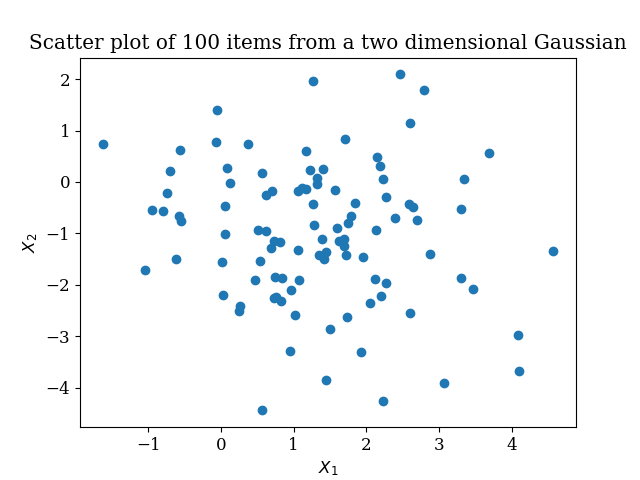
\includegraphics[width=0.6\textwidth]{../images/7_a.png}  
			            % reference folder/figure.pdf here and adjust width
			    \captionsetup{labelformat=empty}
			    \caption{Drawing from a Gaussian distribution}
			    \label{fig:guass}
			\end{figure}
		\end{soln}
	
		\item Make a scatter plot by drawing 100 items from a mixture distribution 
		$0.3 N\left((5, 0)^{T}, \begin{pmatrix} 1 & 0.25 \\ 0.25 & 1\\ \end{pmatrix}\right)
		+0.7 N\left((-5, 0)^{T}, \begin{pmatrix} 1 & -0.25 \\ -0.25 & 1\\ \end{pmatrix}\right)
		$.
		
		\begin{soln}
		% add figure filename, and remove % 
		%    (this can be done by highlighting text and pressing "cmd + /" for sharelatex+mac)
		\begin{figure}[h!]
		    \centering
		    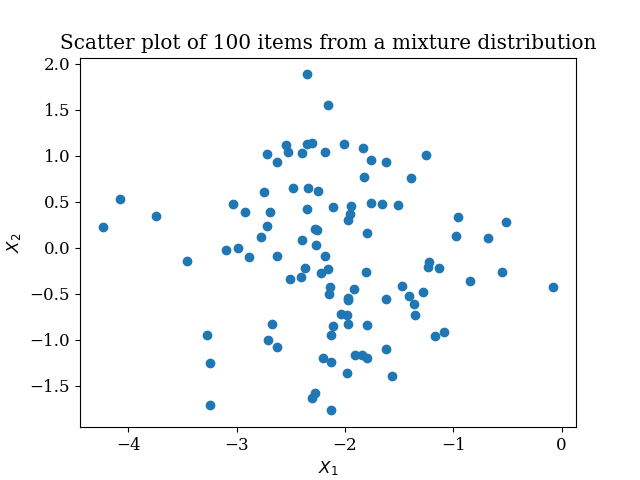
\includegraphics[width=0.6\textwidth]{../images/7_b.png}  
		            % reference folder/figure.pdf here and adjust width
		    \captionsetup{labelformat=empty}
		    \caption{Drawing from a Gaussian mixture distribution}
		    \label{fig:gauss_mixture}
		\end{figure}
	\end{soln}
	\end{enumerate}
	
	
	\bibliographystyle{apalike}
	
	
	%----------------------------------------------------------------------------------------
	
	
\end{document}
